\documentclass[12pt,letterpaper, onecolumn]{exam}
\usepackage{amsmath}
\usepackage{amssymb}
\usepackage[lmargin=71pt, tmargin=1.2in]{geometry}  %For centering solution box
\usepackage[shortlabels]{enumitem}
\usepackage{subcaption}
\usepackage[final]{graphicx}
\usepackage{float}
\lhead{Leaft Header\\}
\rhead{Right Header\\}
% \chead{\hline} % Un-comment to draw line below header
\thispagestyle{empty}   %For removing header/footer from page 1

\begin{document}

\begingroup  
    \centering
    \LARGE Machine Learning: Project\\
    \LARGE Multi-Agent Learning in Canonical Games and Knights Archers Zombies\\[0.5em]
    \large \today\\[0.5em]
    \large Dimitrios Mystriotis - Jan Cichomski\par
    \large r1027781 - r1026448\par
\endgroup
\rule{\textwidth}{0.4pt}
\pointsdroppedatright   %Self-explanatory
\printanswers
\renewcommand{\solutiontitle}{\noindent\textbf{Ans:}\enspace}   %Replace "Ans:" with starting keyword in solution box

\section{\textbf{Task 1:}}

\section{\textbf{Task 2:}}
\subsection{}
\begin{itemize}
    \item A game is in Nash equilibrium when no player can improve their outcome by changing their strategy, if the other player doesn't change their's.
    \item A game is in Pareto Optimal when it is impossible to make a player better off without making the total payoff worse.
\end{itemize}
\begin{enumerate}[(\alph*)]
    \item Stag Hunt:
    \begin{itemize}
        \item Nash Equilibria: (Hare,Hare) and (Stag,Stag)
        \item Pareto Optimal: (Hare,Hare) and (Stag,Stag)
    \end{itemize}
    \item Subsidy game:
    \begin{itemize}
        \item Nash Equilibria: (Subsidy 2,Subsidy 2)
        \item Pareto Optimal: (Subsidy 1,Subsidy 1) and (Subsidy 2,Subsidy 2)
    \end{itemize}
    \item Matching Pennis:
    \begin{itemize}
        \item Nash Equilibria: There is no Nash Equilibria for a pure strategy. For a mixed strategy, the Nash Equilibria is picking heads or tails with probability 0.5 each.
        \item Pareto Optimal: Every outcome is Pareto Optimal
    \end{itemize}
    \item Prisoner's Dilemma:
    \begin{itemize}
        \item Nash Equilibria: (Defect,Defect)
        \item Pareto Optimal: (Cooperate,Cooperate)
    \end{itemize}
\end{enumerate}

\subsection{}

The e-Greedy algorithm converges to the Nash Equilibrium for all games. Even when an algorithm converges to the Pareto Optimal solution, it starts to move towards the Nash Equilibrium
as the number of iterations increases. This is because the Nash Equilibrium is the most stable solution, which random choices will favor. For the learning trajectories of e-Greedy,
the action choice depends on q values and it is picked deterministically. This makes it complicated to plot the learning trajectories, as the probabilities to chose an action are 
constant making it hard to plot a graph. 

The Boltzmann algorithm converges to either the Nash Equilibrium or the Pareto Optimal solution. The Boltzmann algorithm is more likely to converge to the Pareto Optimal solution
compared to the e-Greedy algorithm, and it doesn't deviate from that point. The algorithm will basically find an optimal solution (either Nash or Pareto) and stick to it.
Which on is favored depends on the starting distance from the point and the rewards of the game. It seams to favor the Nash Equilibrium slightly more than the Pareto Optimal solution.

\begin{figure}[H]
    \begin{subfigure}{.5\textwidth}
      \centering
      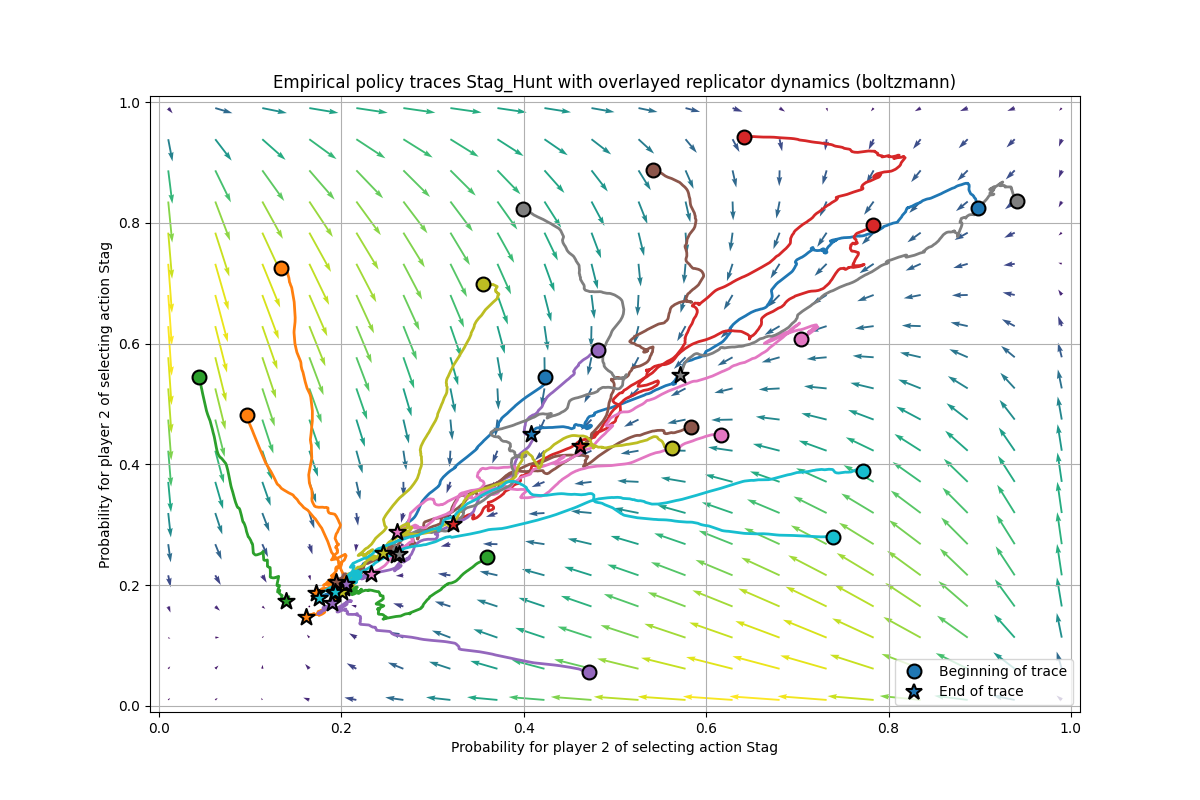
\includegraphics[width=.6\linewidth]{plots/replicator_trajectoreis_Stag_Hunt_boltzmann.png}
      \caption{Boltzmann Q-Learning Stag Hunt}
      \label{fig:sfigbsh}
    \end{subfigure}%
    \begin{subfigure}{.5\textwidth}
      \centering
      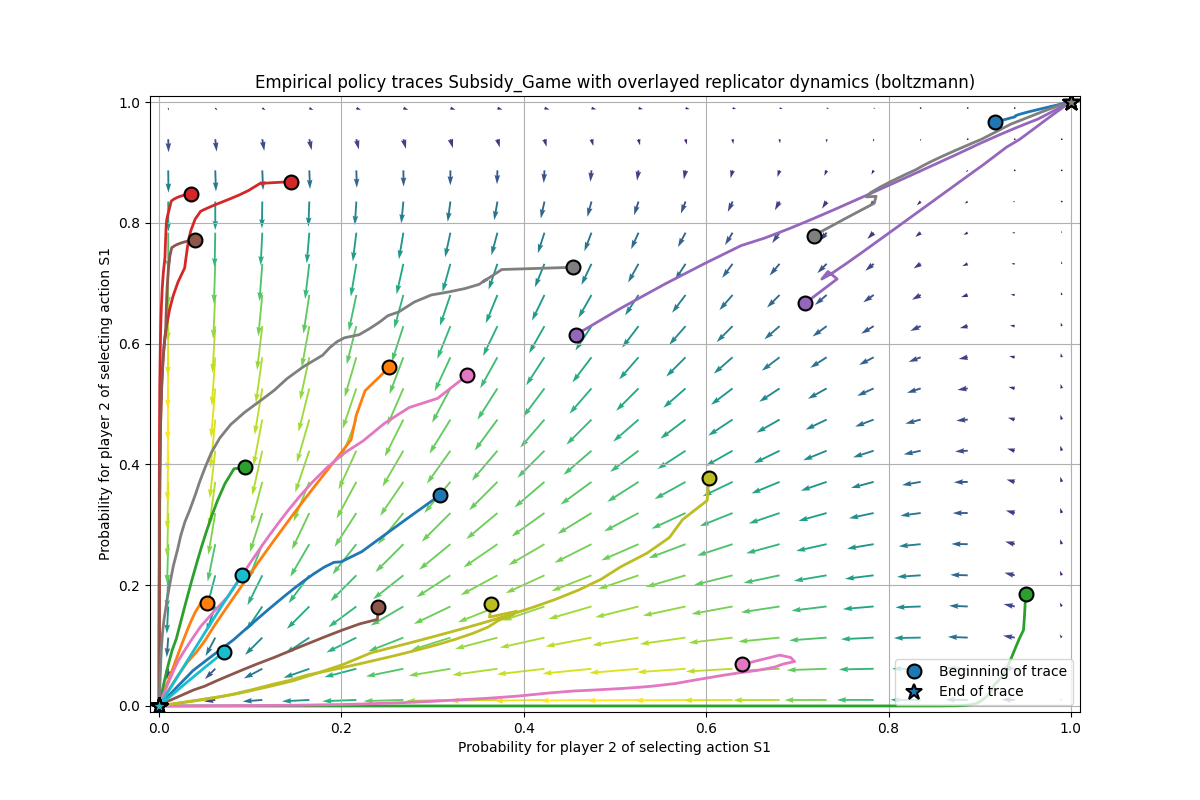
\includegraphics[width=.6\linewidth]{plots/replicator_trajectoreis_Subsidy_Game_boltzmann.png}
      \caption{Boltzmann Q-Learning Subsidy Game}
      \label{fig:sfigbsg}
    \end{subfigure}\\
    \begin{subfigure}{.5\textwidth}
      \centering
      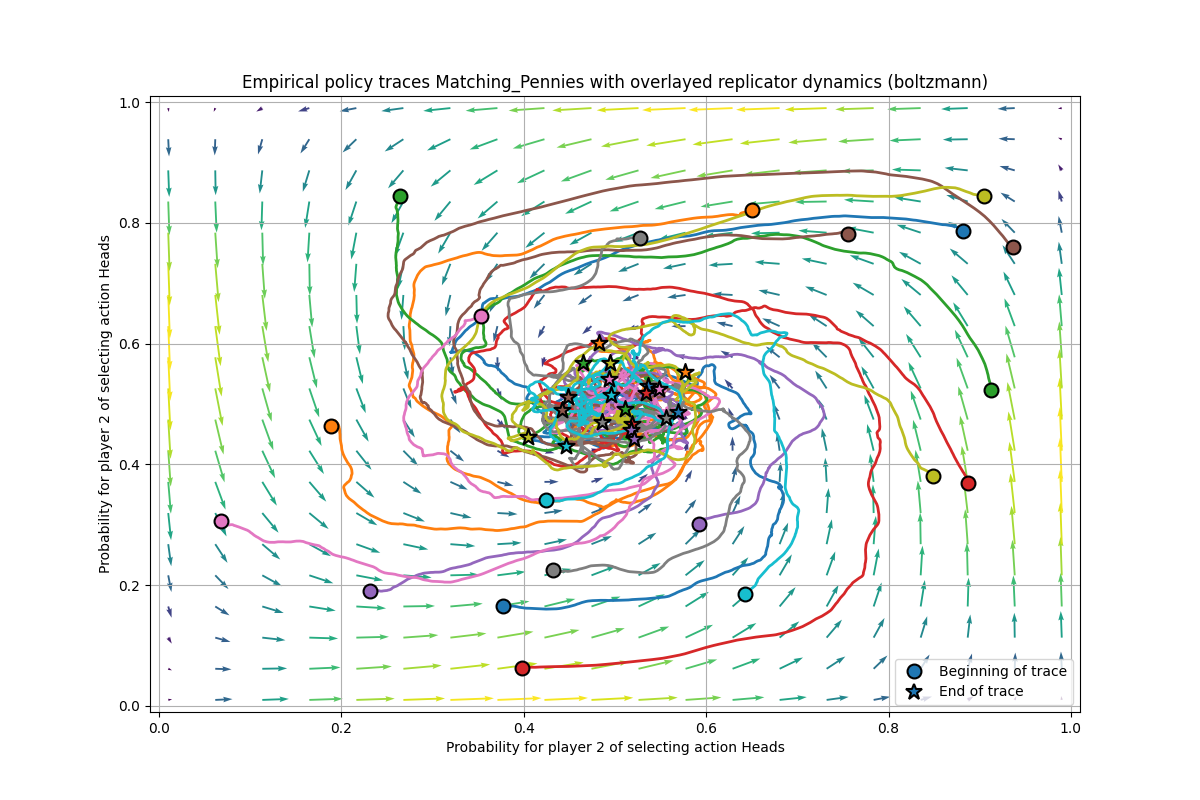
\includegraphics[width=.6\linewidth]{plots/replicator_trajectoreis_Matching_Pennies_boltzmann.png}
      \caption{Boltzmann Q-Learning Matching Pennies}
      \label{fig:sfigbmp}
    \end{subfigure}%
    \begin{subfigure}{.5\textwidth}
      \centering
      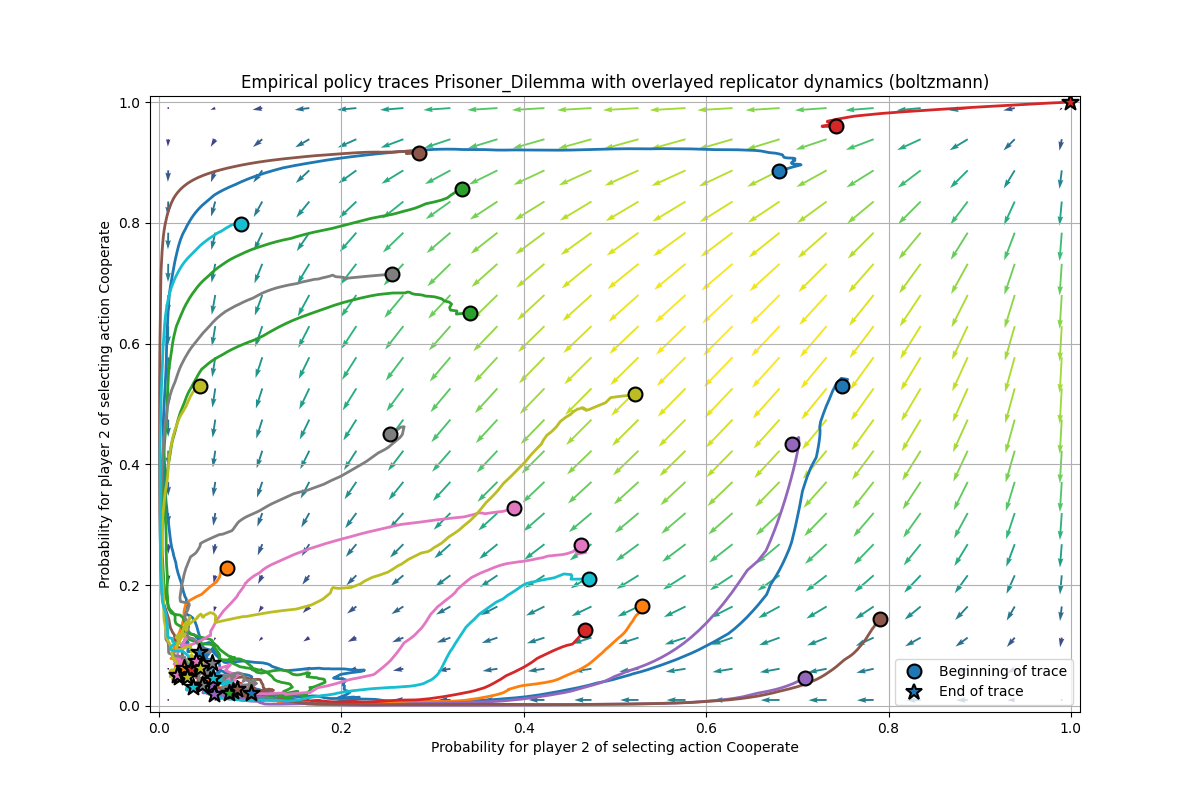
\includegraphics[width=.6\linewidth]{plots/replicator_trajectoreis_Prisoner_Dilemma_boltzmann.png}
      \caption{Boltzmann Q-Learning Prisoner's Dilemma}
      \label{fig:sfigbpd}
    \end{subfigure}%
\end{figure}

For the Lenient Boltzmann Q-Learning algorithm, the results are similar to the Boltzmann Q-Learning algorithm. The main advantage of the Lenient Boltzmann Q-Learning algorithm is that it
evaluates multiple actions when performing an action thus allowing for better exploration of the problem space. This can be seen in the plots, where the algorithm is more likely to explore
the problem space and find the Pareto Optimal solutions. The existence of the k value allow for the algorithm to explore more or less, depending on the value of k.

\begin{figure}[H]
    \begin{subfigure}{.5\textwidth}
      \centering
      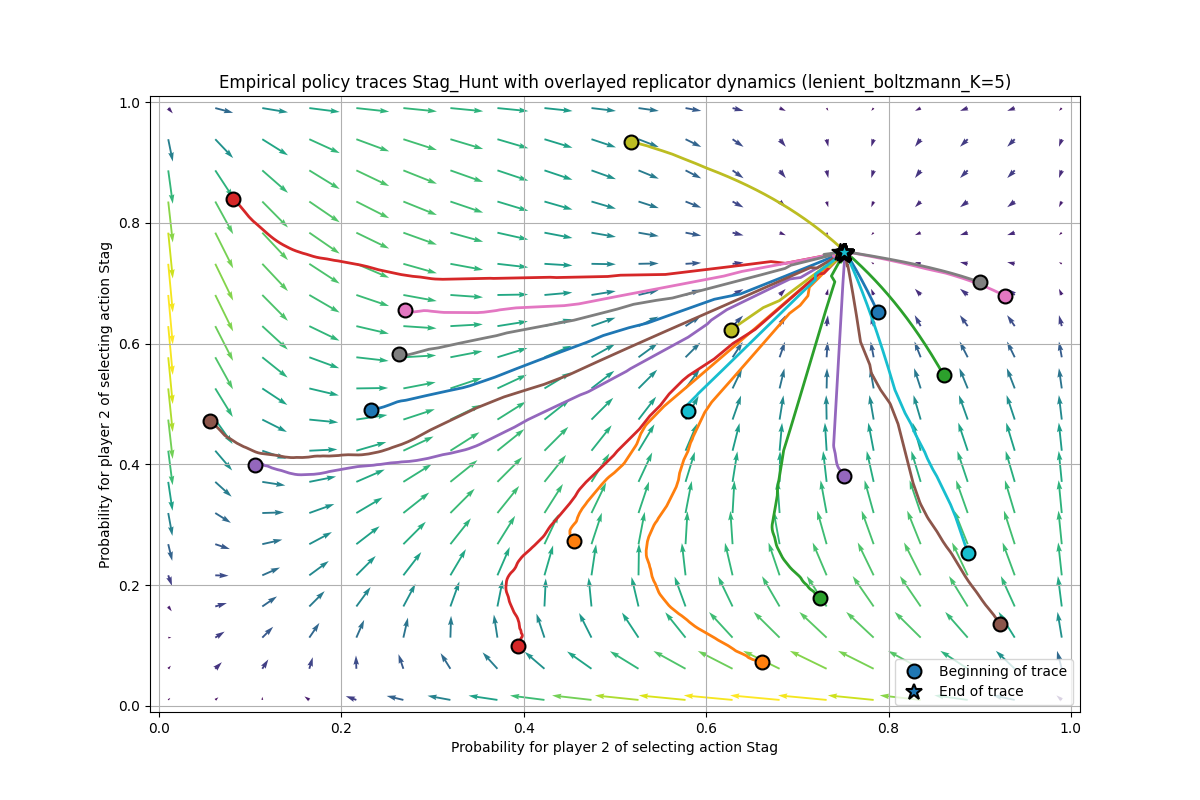
\includegraphics[width=.6\linewidth]{plots/replicator_trajectoreis_Stag_Hunt_lenient_boltzmann_K=5.png}
      \caption{Lenient Boltzmann Q-Learning\\ Stag Hunt}
      \label{fig:sfiglbsh}
    \end{subfigure}%
    \begin{subfigure}{.5\textwidth}
      \centering
      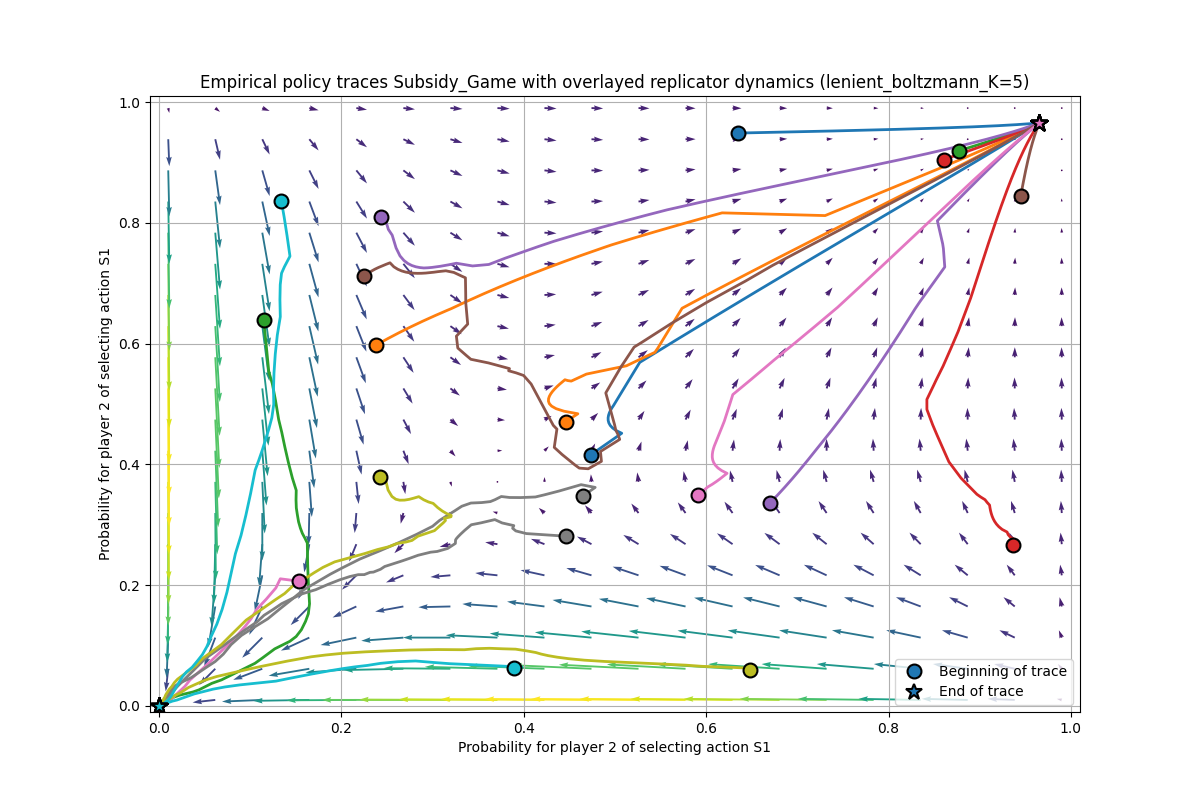
\includegraphics[width=.6\linewidth]{plots/replicator_trajectoreis_Subsidy_Game_lenient_boltzmann_K=5.png}
      \caption{Lenient Boltzmann Q-Learning\\ Subsidy Game}
      \label{fig:sfiglbsg}
    \end{subfigure}\\
    \begin{subfigure}{.5\textwidth}
      \centering
      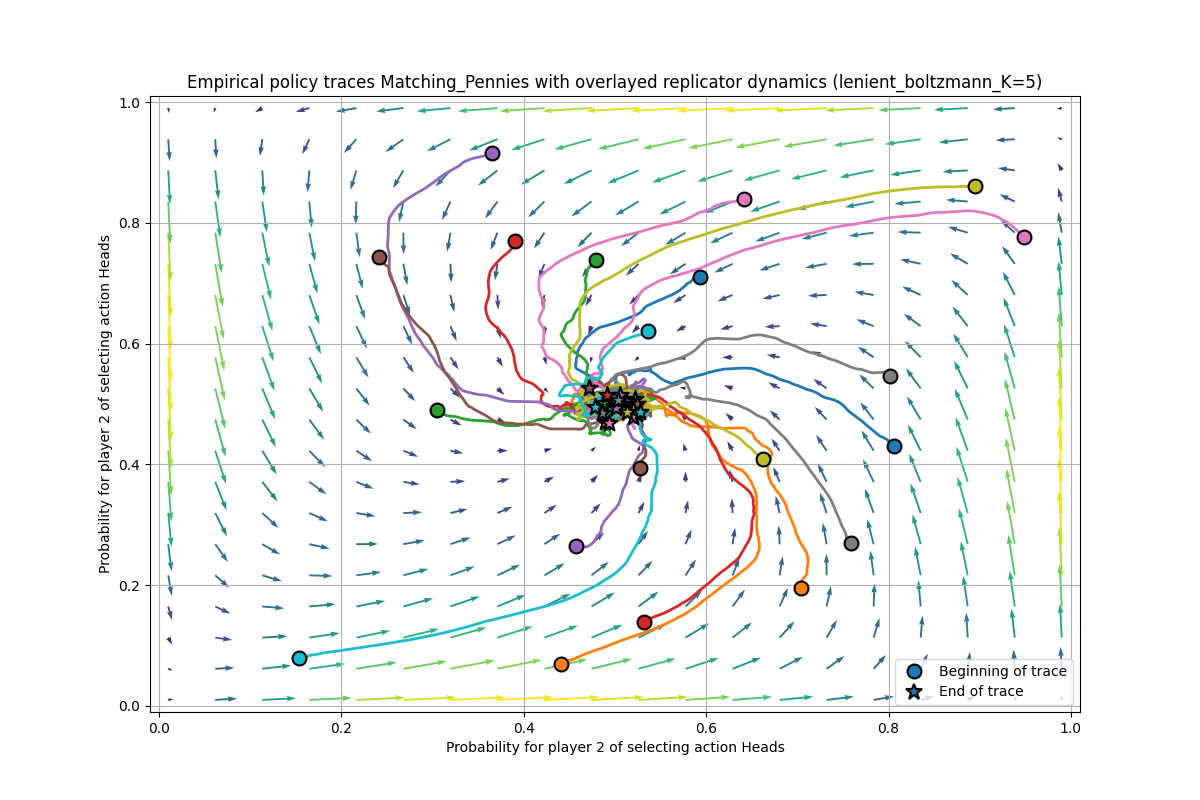
\includegraphics[width=.6\linewidth]{plots/replicator_trajectoreis_Matching_Pennies_lenient_boltzmann_K=5.png}
      \caption{Lenient Boltzmann Q-Learning\\ Matching Pennies}
      \label{fig:sfiglbmp}
    \end{subfigure}%
    \begin{subfigure}{.5\textwidth}
      \centering
      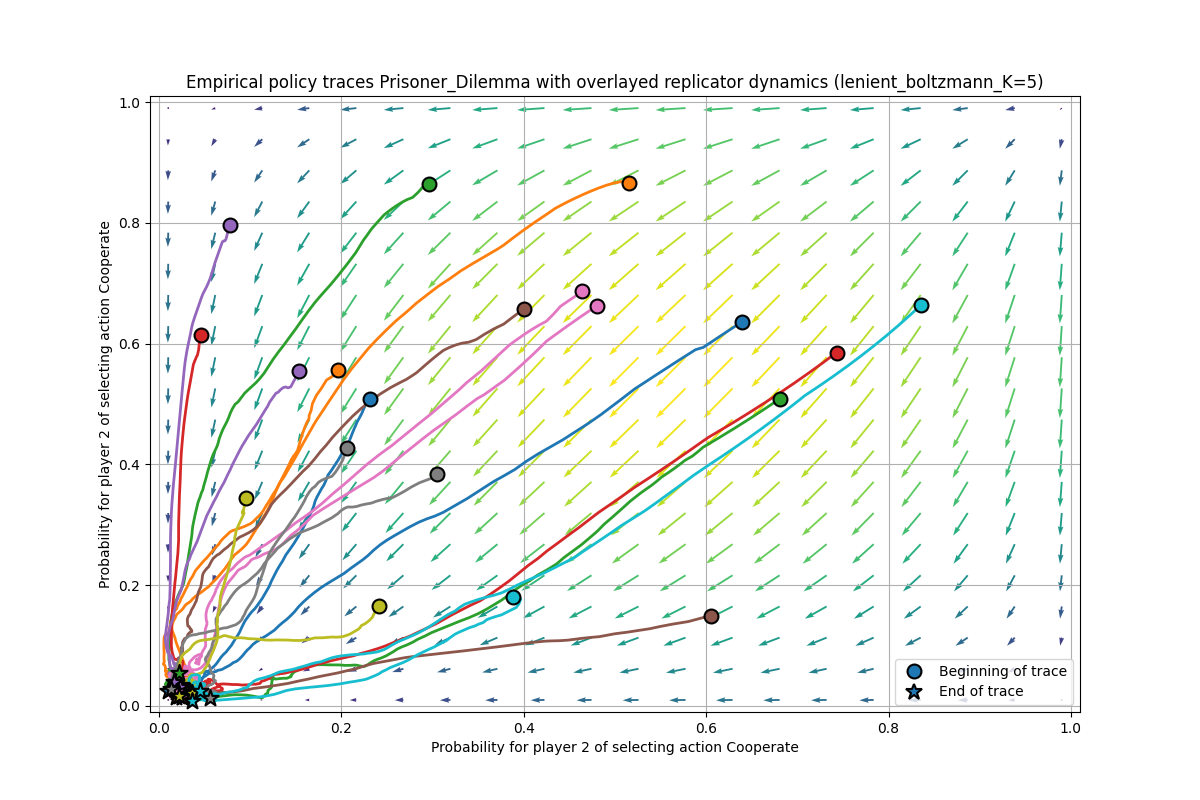
\includegraphics[width=.6\linewidth]{plots/replicator_trajectoreis_Prisoner_Dilemma_lenient_boltzmann_K=5.png}
      \caption{Lenient Boltzmann Q-Learning\\ Prisoner's Dilemma}
      \label{fig:sfiglbpd}
    \end{subfigure}%
\end{figure}

By changing the k value of the Lenient Boltzmann Q-Learning algorithm, the learning trajectories change.
Higher k values provide significantly better results which can be seen in the plots \ref{fig:sfiglbshk1} - \ref{fig:sfiglbshk25}.

\begin{figure}[H]
    \begin{subfigure}{.5\textwidth}
      \centering
      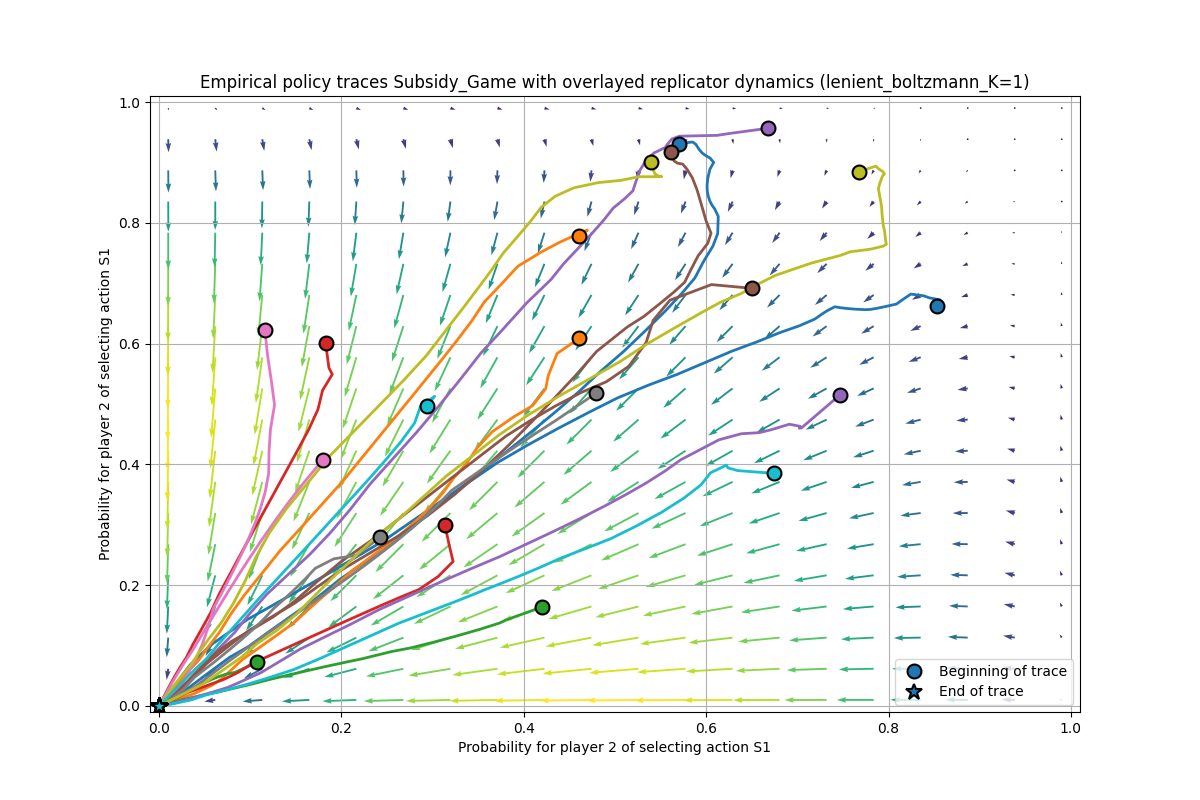
\includegraphics[width=.6\linewidth]{plots/replicator_trajectoreis_Subsidy_Game_lenient_boltzmann_K=1.png}
      \caption{Lenient Boltzmann Q-Learning\\ Subsidy Game (K=1)}
      \label{fig:sfiglbshk1}
    \end{subfigure}
    \begin{subfigure}{.5\textwidth}
      \centering
      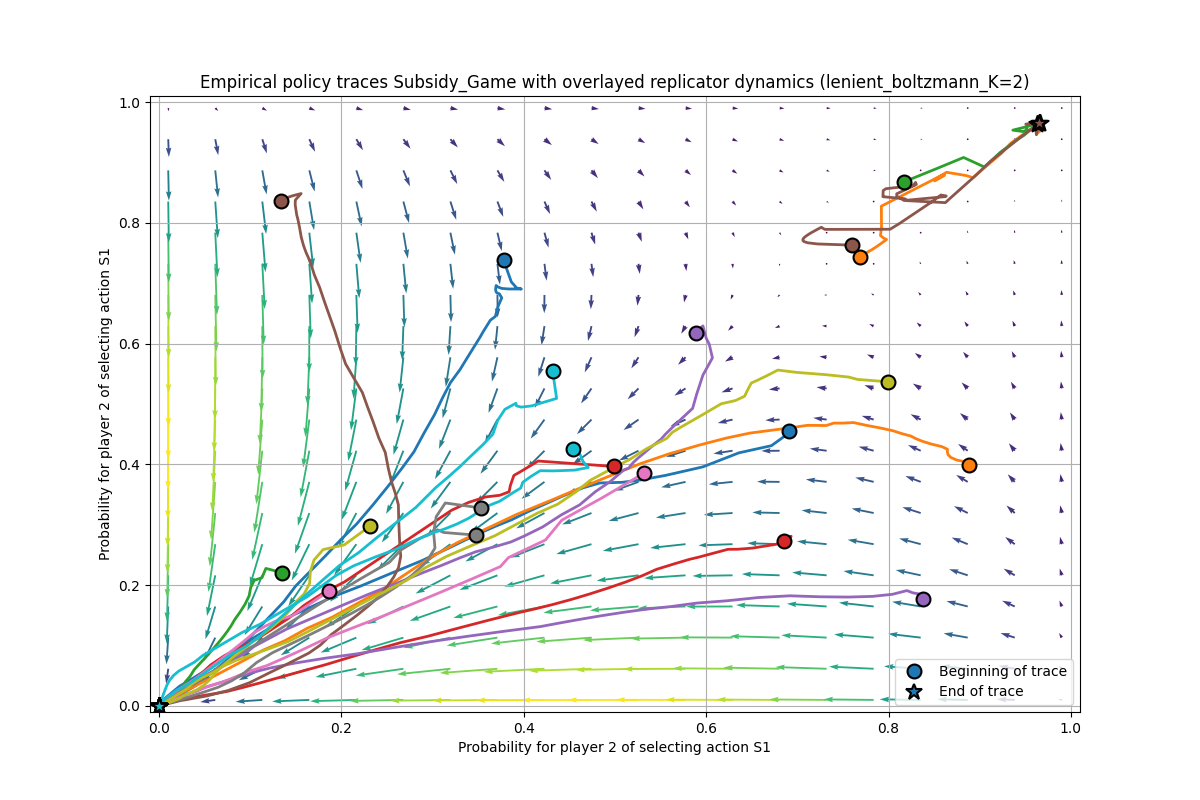
\includegraphics[width=.6\linewidth]{plots/replicator_trajectoreis_Subsidy_Game_lenient_boltzmann_K=2.png}
      \caption{Lenient Boltzmann Q-Learning\\ Subsidy Game (K=2)}
      \label{fig:sfiglbshk2}
    \end{subfigure}\\
    \begin{subfigure}{.5\textwidth}
      \centering
      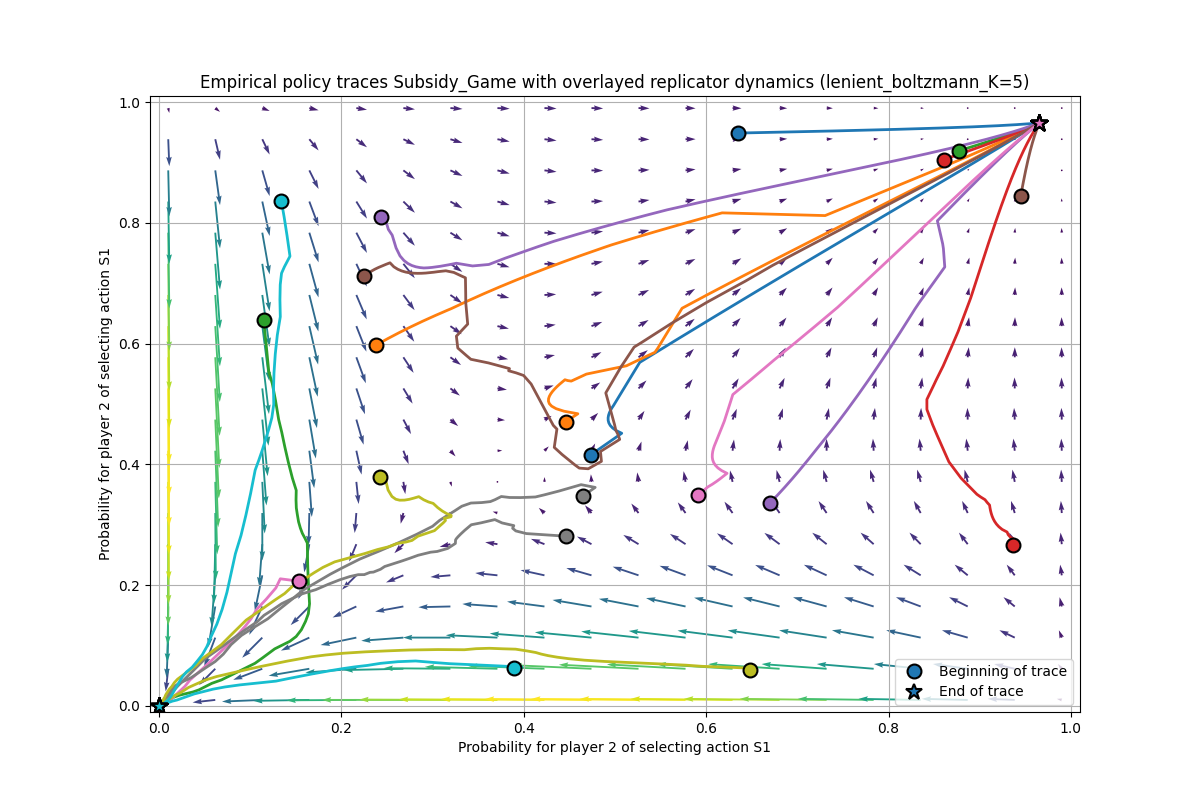
\includegraphics[width=.6\linewidth]{plots/replicator_trajectoreis_Subsidy_Game_lenient_boltzmann_K=5.png}
      \caption{Lenient Boltzmann Q-Learning\\ Subsidy Game (K=5)}
      \label{fig:sfiglbshk5}
    \end{subfigure}
    \begin{subfigure}{.5\textwidth}
      \centering
      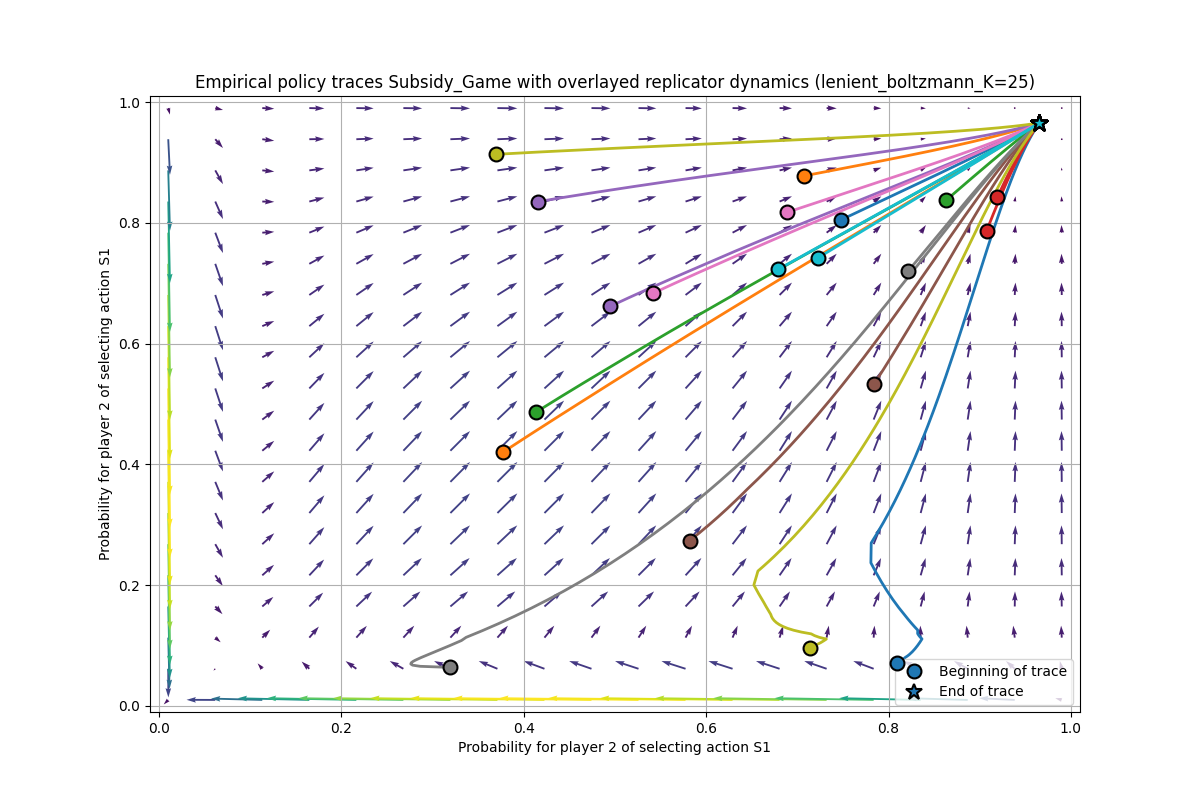
\includegraphics[width=.6\linewidth]{plots/replicator_trajectoreis_Subsidy_Game_lenient_boltzmann_K=25.png}
      \caption{Lenient Boltzmann Q-Learning\\ Subsidy Game (K=25)}
      \label{fig:sfiglbshk25}
    \end{subfigure}
\end{figure}

\subsection{}

The learning trajectories are behaving as expected and do follow the replicator dynamics. For each of the games learning follow the dynamics, especially for the Lenient Boltzmann Q-Learning algorithm
were the changes of the k value affects both dynamics and trajectories making the match between the two very visible. The results can be seen in the figures above \ref{fig:sfiglbshk1} were the
effect of the k value can shift the learning trajectories to converge to a better solution even if it's not the Nash Equilibrium.

\section{\textbf{Task 3:}}

\section{\textbf{Task 4:}}


\end{document}